%%%%%%%%%%%%%%%%%%%%%%%%%%%%%%%%%%%%%%%%%
% "ModernCV" CV and Cover Letter
% LaTeX Template
% Version 1.1 (9/12/12)
%
% This template has been downloaded from:
% http://www.LaTeXTemplates.com
%
% Original author:
% Xavier Danaux (xdanaux@gmail.com)
%
% License:
% CC BY-NC-SA 3.0 (http://creativecommons.org/licenses/by-nc-sa/3.0/)
%
% Important note:
% This template requires the moderncv.cls and .sty files to be in the same 
% directory as this .tex file. These files provide the resume style and themes 
% used for structuring the document.
%
%%%%%%%%%%%%%%%%%%%%%%%%%%%%%%%%%%%%%%%%%

%----------------------------------------------------------------------------------------
%	PACKAGES AND OTHER DOCUMENT CONFIGURATIONS
%----------------------------------------------------------------------------------------

\documentclass[11pt,a4paper,sans]{moderncv} % Font sizes: 10, 11, or 12; paper sizes: a4paper, letterpaper, a5paper, legalpaper, executivepaper or landscape; font families: sans or roman

\moderncvstyle{classic} % CV theme - options include: 'casual' (default), 'classic', 'oldstyle' and 'banking'
\moderncvcolor{purple} % CV color - options include: 'blue' (default), 'orange', 'green', 'red', 'purple', 'grey' and 'black'
%\usepackage[italian]{babel}
\usepackage[utf8]{inputenc}
\usepackage{lmodern}
\usepackage{enumitem}
\usepackage{fontawesome5}
\usepackage{ragged2e}
\usepackage{graphicx}
\usepackage{wrapfig}

\usepackage[scale=0.9, top=1cm, bottom=1cm, left=0.7cm, right=0.7cm]{geometry} % Reduce document margins
\setlength{\hintscolumnwidth}{4cm} % Uncomment to change the width of the dates column
%\setlength{\makecvtitlenamewidth}{10cm} % For the 'classic' style, uncomment to adjust the width of the space allocated to your name

%----------------------------------------------------------------------------------------
%	NAME AND CONTACT INFORMATION SECTION
%----------------------------------------------------------------------------------------

\firstname{Francesco} % Your first name
\familyname{Dondi} % Your last name

% All information in this block is optional, comment out any lines you don't need
\title{A Florence on raconte \\ \hfill que la Terre serait ronde}
\mobile{+41 76456 50 32\hfill\ }
\email{francesco314@gmail.com\hfill\ }
\social[linkedin]{francesco-dondi\hfill\ }
\social[github]{Fdondi\hfill\ }
\address{Resident 8810 Horgen, Zürich canton \hfill\ }
\extrainfo{\faIcon{birthday-cake} Born 1990, Italy, Italian citizen\hfill\  \\ \faIcon{plus-square} Swiss C permit until 30.09.27 \hfill\ \\ \faIcon{globe} German B2 planned Mar 2024\hfill\ }
\photo[100pt][0pt]{me.jpg} % The first bracket is the picture height, the second is the thickness of the frame around the picture (0pt for no frame)

%----------------------------------------------------------------------------------------

% Store the old definition of \makecvtitle
\let\oldmakecvtitle\makecvtitle

% Redefine \makecvtitle based on the old definition
\renewcommand*{\makecvtitle}{%
  \hfil% push content to the right
  \oldmakecvtitle%
}

\newcommand{\ToolList}[1]{
\hfill
\begin{minipage}[t]{0.15\textwidth}
{\tiny
  \begin{itemize}
    \setlength\itemsep{-0.3em}
    #1
  \end{itemize}
}
\end{minipage}
}

\begin{document}

\makecvtitle % Print the CV title
\vspace{-10mm}
\begin{minipage}{0.5\linewidth}
\vspace{7mm}
\section{Professional Experience}
\end{minipage}
\begin{minipage}{0.5\linewidth}
  \centering
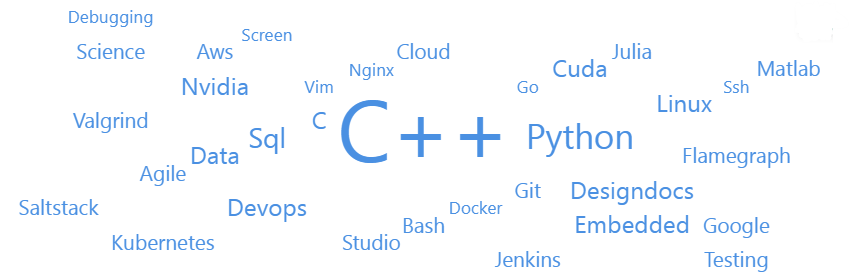
\includegraphics[width=0.7\textwidth]{cloud_long.png}
\vspace{-4mm}
\end{minipage}
\cventry{03/2023 - 09/2023 \\ \textbf{DoubleCloud}}{Software Developer}{}{Fully Remote}{}{
\noindent
\begin{minipage}[t]{0.65\textwidth}
Maintained and developed the infrastructure around managed ClickHouse, in particular:
\begin{itemize}
\setlength\itemsep{-0.3em}
\item Secured metrics server by adding Nginx
\item Improved SaltStack configuration
\item Solved bugs in Telegraf Go plugins
\end{itemize}
\end{minipage}
\ToolList{
	\item \faPencil*{} C++
	\item \faPencil*{} Go
	\item \faPencil*{} Bash
    \item \faDatabase{} ClickHouse SQL
	\item \faCodeBranch{} Git
	\item \faLinux Linux, Bash
}
\ToolList{
	\item \faCloud{} AWS storage
	\item \faCog{} Docker
	\item \faCog{} Jenkins CI
	\item \faCog{} Nginx
	\item \faCog{} SaltStack
}
}

\cventry{06/2021 - 09/2022 \\ \textbf{Firebolt}}{Software Developer}{}{Fully Remote}{}{
\noindent
\begin{minipage}[t]{0.65\textwidth}
Maintained and developed the SQL optimization engine and testing infrastructure.
\begin{itemize}
\setlength\itemsep{-0.3em}
\item Expanded supported SQL syntax and optimizations
\item reworked the test framework to support new test suite
\item contributed to rewriting to higher standards the optimization engine 
\end{itemize}
\end{minipage}
\ToolList{
	\item \faPencil*{} C++
	\item \faPencil*{} Python
    \item \faDatabase{} Firebolt SQL
	\item \faCodeBranch{} Git
}
\ToolList{
	\item \faBrain{} Testing
	\item \faCog{} Jenkins
    \item \faBrain{} Debugging
    \item \faCloud{} AWS storage    
}
}

\cventry{08/2020 - 02/2021 \\ \textbf{F-Trust}}{Developer / Analyst}{}{Zug / 50\% Remote}{}{
\noindent
\begin{minipage}[t]{0.65\textwidth}
\begin{itemize}
\setlength\itemsep{-0.3em}
\item Maintained and developed a Trading Engine (C++)
\item redesigned, implemented and migrated product storage (PostgreSQL)
\item extracted and integrated data from multiple log streams
\item analyzed said data to highlight opportunities for improvement (Julia)
\end{itemize}
\end{minipage}
\ToolList{
	\item \faPencil*{} C++
	\item \faPencil*{} Julia
    \item \faDatabase{} PostgreSQL
	\item \faCodeBranch{} Git
	\item \faBrain{} Data Science
}
\ToolList{
	\item \faLinux Linux
	\item \faLinux Bash
	\item \faLinux SSH
	\item \faLinux VIM
	\item \faLinux \href{https://linuxize.com/post/how-to-use-linux-screen/}{Screen}
}
}

\cventry{10/2017 - 05/2020 \\ \textbf{Google}}{Software Developer}{}{Zürich / 10\% Remote}{}{
\noindent
\begin{minipage}[t]{0.65\textwidth}
Within Search, productionized an initially experimental tool (C++).
\begin{itemize}
\setlength\itemsep{-0.3em}
\item Improved runtime from days to hours
\item added support for new kinds of data
\item made the results easily visualizable and monitorable
\item made onboarding orders of magnitude faster for most cases
\end{itemize}
\end{minipage}
\ToolList{
	\item \faPencil*{} C++ [Abseil]
	\item \faPencil*{} Python
    \item \faDatabase{} Google SQL
	\item \faCodeBranch{} ~internal~
    \item \faCog{} Valgrind
	\item \faCog{} Flamegraph
}
\ToolList{
	\item \faBrain{} DevOps
	\item \faBrain{} Design Docs
	\item \faLinux{} Linux
	\item \faPencil*{} Bash
	\item \faCog{} Kubernetes
	\item \faCog{} \href{https://marketingplatform.google.com/about/data-studio/}{Google Data Studio} 
}
}
\cventry{04/2016 - 10/2017 \\ \textbf{Ascent Software}}{Software Developer}{}{Luqa(Malta)}{}{
\noindent
\begin{minipage}[t]{0.65\textwidth}
Bridging from internal API to new device API for automotive.
\end{minipage}
\ToolList{
	\item \faPencil*{} C++ [Boost]
	\item \faBrain{} Embedded development
	\item \faWindows Windows
}
\ToolList{
    \item \faBrain{} Agile development
	\item \faCodeBranch{} Git
	\item \faWindows Visual Studio
}
}


\cventry{04/2015 - 04/2016 \\ \textbf{Rulex Inc.}/\textbf{CNR}}{Junior Developer}{}{Genua (Italy)}{}{
\noindent
\begin{minipage}[t]{0.65\textwidth}
Reworked C/MATLAB algorithms for OpenMP/CUDA parallelization
\end{minipage}
\ToolList{
	\item \faPencil*{} C
	\item \faCog{} Nvidia CUDA
	\item \faWindows Windows
} 
\ToolList{
    \item \faPencil*{} MATLAB
    \item \faPencil*{} Python
    \item \faWindows Visual Studio
}
}

\section{Education}

\subsection{Formal education}

\cventry{2023 H1}{\href{https://execed-online.imperial.ac.uk/business-analytics}{From Data to Decisions}}{Imperial College Business School}{}{}{}
\cventry{2009--2015}{\href{http://www.unipd-scuolagalileiana.it/en/}{Galileian School of Higher Education}}{University of Padua}{Enriching program for gifted students}{\textit{98/100}}{}
\cventry{2012--2014}{Master Degree in Mathematics}{University of Padua}{}{\textit{108/110}}{}
\cventry{2009--2012}{Bachelor Degree in Mathematics}{University of Padua}{}{\textit{110/110 cum Laude}}{}
\cventry{2004--2009}{High School - Science Track, with added French and IT}{Liceo E. Fermi}{Bologna}{\textit{100/100 cum Laude}}{}

\pagebreak

\subsection{Continuous Learning}

\cventry{Nov 2023}{Business Intelligence for Consultants}{Linkedin}{Gini von Courter}{3h 45m}{
\begin{minipage}[t]{0.65\textwidth}
Data types in Power BI. Visualizations in Power BI. Outcomes when changes are made within Power BI and Power BI Desktop. Dashboards vs reports within Power BI. User roles within a workspace in Power BI.
Workspaces and tools within the Power BI mobile application.
\end{minipage}
\ToolList{
	\item \faBrain{} Microsoft Power BI 
}
\ToolList{	
	\item \faBrain{} Data Visualization
}
}

\cventry{Oct 2023}{Business Intelligence for Consultants}{Linkedin}{Joshua Rischin}{29m}{
\begin{minipage}[t]{0.65\textwidth}
Determine the essentials of business needs. Recognize the fundamentals in reviewing source data. Break down the meaning behind data-driven insights.
\end{minipage}
\ToolList{
	\item \faBrain{} Business Intelligence
}
\ToolList{	
	\item \faBrain{} Data Visualization
}
}

\cventry{Oct 2023}{Data Analytics for Business Professionals}{Linkedin}{John Johnsond}{1h 16m}{
\begin{minipage}[t]{0.65\textwidth}
Explore examples of real-life analytics in action, distinguishing between predictive and prescriptive approaches, and learning how to formulate and pose your own questions. Find out how to collect, clean, and aggregate data from different sources across your organization, and identify when data is flawed.
\end{minipage}
\ToolList{
	\item \faCog{} Pandas	
	\item \faCog{} Databases
}
\ToolList{	
	\item \faBrain{} Data Analytics
	\item \faBrain{} Data Visualization
}
}


\cventry{Oct 2023}{Excel: Economic Analysis and Data Analytics}{Linkedin}{Michael McDonald}{2h 17m}{
\begin{minipage}[t]{0.65\textwidth}
Using regression analysis, confidence intervals, and forecasting tools with your company’s key performance indicators (KPIs), building your skill set in data analytics to better meet the needs of your business.
\end{minipage}
\ToolList{
	\item \faCog{} Microsoft Excel	
	\item \faBrain{} Economic Analysis
}
\ToolList{
	\item \faBrain{} Data Analytics
	\item \faBrain{} Data Visualization
}
}

\cventry{Oct 2023}{The Non-Technical Skills of Effective Data Scientists}{Linkedin}{Keith McCormick}{44m}{
\begin{minipage}[t]{0.65\textwidth}
New data scientists must be able to empathize, persuade, and lead others if they want to successfully run projects that produce business transformation.
\end{minipage}
\ToolList{
	\item \faBrain{} Business communication
}
\ToolList{
	\item \faBrain{} Data Science
}
}

\cventry{Oct 2023}{Learning MATLAB}{Linkedin}{Steven Moser}{1h 13m}{
\begin{minipage}[t]{0.65\textwidth}
How to harness the MATLAB tools and create programs to model your own data and hypotheses
\end{minipage}
\ToolList{
	\item \faPencil*{} MATLAB 
}
\ToolList{
	\item \faBrain{} Data Processing 
}
}

\cventry{Feb 2023}{AWS Certified Solutions Architect - Associate (SAA-C02) Cert Prep: 1 Cloud Services Overview}{Linkedin}{Tom Carpenter}{1h7m}{
\begin{minipage}[t]{0.65\textwidth}
Explore the benefits of cloud computing, the range of AWS services, the security solutions built into AWS, and the AWS regions and availability zones.
\end{minipage}
\ToolList{
	\item \faCog{} AWS Cloud 
}
\ToolList{
	\item \faBrain{} Cloud Computing 
}
}

\cventry{Jan 2023}{DevOps Foundations: Going Cloud Native}{Linkedin}{Karthik Gaekwad}{45m}{
\begin{minipage}[t]{0.65\textwidth}
The information senior executives —CTOs, vice presidents, and chief architects— need to know to embrace cloud native.
\end{minipage}
\ToolList{
	\item \faBrain{} DevOps 
}
\ToolList{
	\item \faBrain{} Cloud Development 
}
}

\section{Language}

\cvitemwithcomment{Italian}{Mother tongue}{}
\cvitemwithcomment{English}{Advanced}{110/120 TOEFL, daily use}
\cvitemwithcomment{German}{Intermediate}{B2 level planned from Mar 2024}
\cvitemwithcomment{French}{Good}{}
\cvitemwithcomment{Arabic}{Beginner}{Wife teaching me}


\section{More}
{\small

\subsection{Awards}

\cvitem{2014}{ GRE test score: Verbal 165 ($95^\circ$ percentile), Quantitative : 170 ($98^\circ$ percentile), Analytical: 4.0 ($56^\circ$ percentile }
\cvitem{2009}{Italian Olympics of Mathematics: Gold}
\cvitem{2008}{Italian Olympics of Information Technology: Bronze}
\cvitem{2006}{Special mention in high school literary prize ``Le ali dell'Ippogrifo''}

\subsection{Hackatons}

\cvitem{12-13/12/15}{\href{https://www.h-farm.com/en}{H-Farm} H-Ack Luxottica: ideas for the future of glasses. } 
\cvitem{19-20/03/16}{\href{https://www.h-farm.com/en}{H-Farm} H-Ack Food: reinventing the 'Bio food' experience. }
}
\end{document}
